
%%%%%%%%%%%%%%%%%%%% file icsc2017_template.tex %%%%%%%%%%%%%%%%%%%%%
%
% This is the LaTeX source for the instructions to authors using
% the LaTeX document class 'llncs.cls' for contributions to
% the Lecture Notes in Computer Sciences series.
% http://www.springer.com/lncs       Springer Heidelberg 2006/05/04
%
% It may be used as a template for your own input - copy it
% to a new file with a new name and use it as the basis
% for your article.
%
% NB: the document class 'llncs' has its own and detailed documentation, see
% ftp://ftp.springer.de/data/pubftp/pub/tex/latex/llncs/latex2e/llncsdoc.pdf
%
%%%%%%%%%%%%%%%%%%%%%%%%%%%%%%%%%%%%%%%%%%%%%%%%%%%%%%%%%%%%%%%%%%%


\documentclass[runningheads,a4paper]{llncs}

\usepackage{amssymb}
\setcounter{tocdepth}{3}
\usepackage{graphicx}
% \usepackage{url}
\usepackage{hyperref}
\hypersetup{hidelinks}
\usepackage{listings}
%\usepackage{float}
%\restylefloat{figure, lstlisting} 


\newcommand{\keywords}[1]{\par\addvspace\baselineskip
\noindent\keywordname\enspace\ignorespaces#1}

\pagestyle{headings}
% !TeX spellcheck = en_US 

\addtolength{\textfloatsep}{-15px}
\addtolength{\intextsep}{-5px}

\begin{document}

\mainmatter  % start of an individual contribution

% first the title is needed
\title{Frequency Modulation with Feedback in Granular Synthesis}

% a short form should be given in case it is too long for the running head
\titlerunning{FM with Feedback in GS}


% TO GARANTEE THE DOUBLE BLIND REVIEW PROCESS, PLEASE
% KEEP THESE GENERIC AUTHOR NAMES AND INSTITUTIONS

\author{Øyvind Brandtsegg, Victor Lazzarini}
%

\institute{Norwegian University of Science and Technology, Maynooth University \\ \email{oyvind.brandtsegg@ntnu.no, victor.lazzarini@mu.ie}}



\maketitle

\begin{abstract}

The paper investigates audio synthesis with frequency modulation feedback in granular synthesis, comparing it with regular FM feedback. 

\keywords{...}
\end{abstract}


\section{Introduction}
FM synthesis is well known ..., FM feedback has been explored by (Lazzarini 2024),...here we will look at FM with feedback within granular synthesis as it allows some new means of pitch stabilisation, poses some new problems, and enables some exciting new sonic extensions to both FM and granular synthesis domains.

\section{Basis for comparison}
FM feedback with oscillators and FM feedback in granular synthesis are closely related. Both techniques use a wavetable-reading oscillator to create the output waveform, and the frequency of reading the waveform in the table is modulated by the output waveform via feedback. Granular synthesis differ from the simpler oscillator case in that the wavetable-reading process is reinitialized on every grain, and that an envelope is applied to each grain. The envelope applied to grains can be seen as a form of amplitude modulation, with the envelope shape being used as the modulator waveform. As we shall see, the grain duration has a significant effect on the feedback modulation. The reinitialization of wavetable reading on each grain also means we can have a periodic phase reset. Phase considerations can have a significant effect on feedback modulation, as we will also see later when we apply a phase delay in the modulation feedback loop.

\subsection{Basics for comparison}
To enable a comparison between the two techniques, we have attempted to create parameter settings for the granular synthesizer that as close as possible resemble the output from a simple oscillator. In that situation, we can compare differences in parameter settings that apply to both synthesis models. Then, from that comparable situation, we can start to apply parameter changes to the granular process that are not available in the simple oscillator model. By doing this, we can explore in specifics how the granular model extends the notion of FM feedback in the granular domain.

In granular synthesis, the perceived pitch is constituted by the grain rate (ref Roads 2001, Brandtsegg 2011). We have thus chosen to let the grain rate be equal to the fundamental frequency of the simple oscillator. Similarly, it makes sense in this context to set the grain frequency (reading speed of the waveform inside each grain) equal to this fundamental frequency. With a the proper envelope, this should allow the granular generator to generate an identical signal as the simple oscillator. The envelope needs to have a smooth fade in and out, and there need to be sufficient overlap between grains to create a constant amplitude in the output. These constraints can be fulfilled in several different ways. With the constraint that the grain rate should equal to the fundamental frequency, the options for the envelope are more limited. We have chosen to use a grain duration of 1.5/grainrate, which means that we have a grain overlap of 33\% (1/3 of the grain will overlap with the next grain). We then use 1/3 of the grain duration for fade in, and equally 1/3 of the duration for fade out. In between fade in and fade out, each grain has a full power sustain period of 1/3 of the grain duration. With an equal power crossfade, we should then be able to recreate a (non granular) waveform. A sigmoid shape is used for the fade in and out of the envelope, to enable equal power crossfading between grains. 

FM feedback with simple oscillators will in its simplest form induce pitch drift, as the output waveform modulate the frequency of the oscillator. This pitch drift can be partly counteracted by recent developments in FM theory (\cite{Lazzarini-2024}), but as this involves an extra step of processing, we don't use it for the simplest possible comparison setup. We will use it as parametric variation when we explore being the simplest possible comparison. The pitch drift can also partly be neutralized by adjusting the phase of the feedback modulator. In feedback modulation, adjusting the phase can be done by introducing a small delay in the feedback signal chain. In audio processing the smallest possible feedback delay is 1 sample, so there is inevitably a delay in the feedback in any case. Also, the adjustment of phase of oscillators can be seen as already existing in the simple FM oscillator configuration. Even if it for us will include an extra processing step (the delay), we consider it to be not more complex than an oscillator with phase control. The delay time is adjusted with respect to the fundamental frequency, so we could call is a phase synced delay. For this reason, delay times are given in fractions of a cycle of the fundamental frequency. 

In our first example we will try to set the parameters so that we get a similar, or comparable, sound from both synthesis models. The example uses an increasing modulation index over time. As can be seen in \ref{fig:simplest}, the sidebands show a similar evolution over time. The first sidebands (over the first 1.5 seconds) appear slightly earlier in the oscillator model, but the break to subharmonics (octaviaton) occurs earlier in the granular model (at 1.7 seconds, similarly at 2.7 seconds in the oscillator model). The transition to chaotic behavior occurs almost simultaneously in both models (around 3.5 second). The synthesis models use a set of default parameters listed in \ref{lst:defaultparameters}, parameter settings deviating from the default setting are listed directly in the figure as nondefault parameters (in between the plots for the granular and oscillator models). The plots show a spectrogram and also zoomed-in snapshots of the waveform at selected locations. The waveform display shows 4 cycles of the waveform in each snapshot, with snapshots being taken every 0.5 seconds of the sound.

\begin{figure}
	\centering
	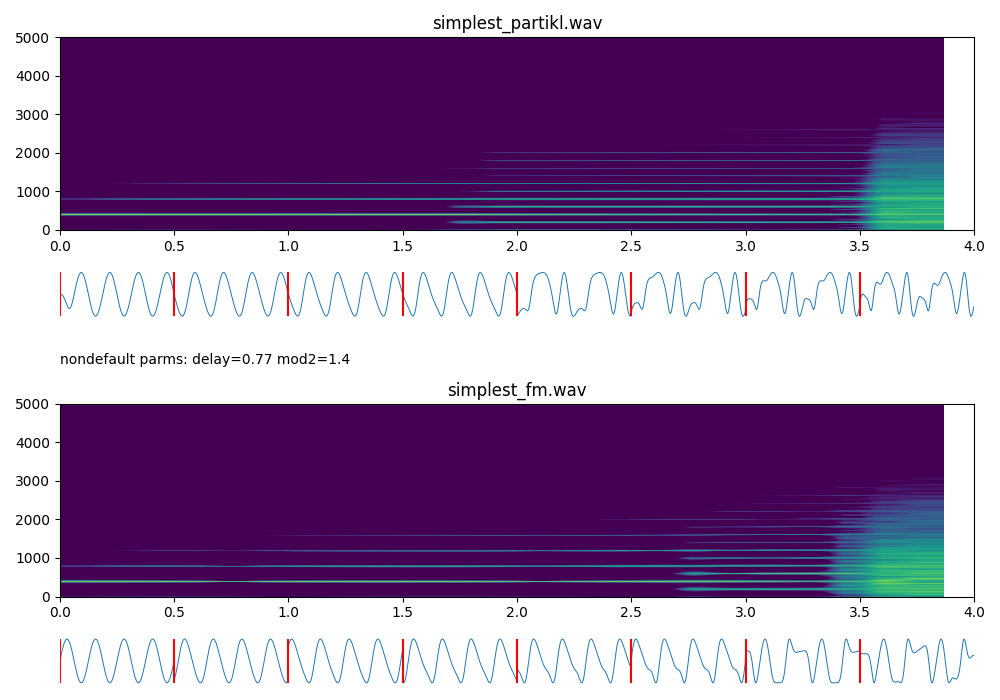
\includegraphics[width=.95\textwidth]{simplest_comparison.png}
	\caption{Creating a similar FM feedback sound with the oscillator model and granular model}
	\label{fig:simplest}
\end{figure}

\noindent\begin{minipage}{\linewidth}
\begin{lstlisting}[caption=Default parameters for the synthesis models, label=lst:defaultparameters]
"dur" = 4 # duration of the generated sound
"amp" = -6 # overall amplitude
"cps" = 400 # fundamental frequency 
"mod1" = 0 # modulation index at start of sound
"mod2" = 1.5 # modulation index at end of sound
"delay" = 0 # phase delay for the feedback modulator
"lpfq" = 21000 # lowpass filter frequency for the feedback modulator 
"hpfq" = 0 #high pass filter frequency for the feedback modulator 
"am" = 0 # enable amplitude modulation on the feedback modulator
"gr.pitch" = 400 # grain frequency 
"gr.dur" = 1.5 # grain duration relative to grain rate
"adratio" = 0.5 # attack to decay ratio of the grain envelope
"sustain" = 0.33 # sustain length for the grain envelope
"index_map" = 0 # modulation index scaling relative to grain duration
"inv_phase2" = 0 # invert the phase of every second grain
maxfreq = 5000 # maximum frequency for the displayed spectrogram
\end{lstlisting}
\emph{Comments to the default parameters
	fundamental frequency (= grain rate for the granular model)
	amplitude modulation on the feedback modulator
	(bypass filter if > 20000)
	(bypass filter if < 0.1)
	(valid only for the granular model(), as are the next 5 parameters)
	also doubles the effective grain rate}
\end{minipage}


\section{Running the provided code examples}
The code examples for this paper can be found in a github repository at \url{https://github.com/Oeyvind/partikkel_fm}. There are Csound orchestra files for FM with granular synthesis and with regular oscillators. To compare the two techniques, it is useful to run both with the same set of parameters (adding only a few extra parameters for granular synthesis), and then compare the generated sound files. The repo contains python files to write score files and render sound with both techniques. This will also display spectrograms for the two generated sound files. The Python files contain default parameter settings as a starting point, and allow parameter modification via command line arguments. For example:
\begin{lstlisting}
python generate_and_compare.py soundfilename cps=200 gr.rate=200
\end{lstlisting}
will modify the fundamental frequency (cps) by setting it to 200Hz, then render sound with both synthesis techniques and display spectrograms for both generated sound files. 

\section{Conclusion}
...

%\pagebreak
\begin{thebibliography}{4}


\bibitem{Brandtsegg-particle} Brandtsegg, Ø. and Saue, S. and Johansen, T. (2011) \emph{Particle synthesis–a unified model for granular synthesis}. Proceedings of the 2011 Linux Audio Conference. \url{http://lac.linuxaudio.org/2011/papers/39.pdf}

\bibitem{Cabbage-url} Walsh, R. \emph{Cabbage - A framework for audio software development.} \url{https://cabbageaudio.com}

\bibitem{Lazzarini-2016} Lazzarini, V. et al. (2016). \emph{Csound: A Sound and Music Computing System.} Springer.

\bibitem{Lazzarini-2024} Lazzarini, V. and Timoney, J. \emph{Theory and Practice of Higher-Order Frequency Modulation
Synthesis}


\end{thebibliography}



\end{document}
